\chapter{Moving target platform landing simulation video description}\label{app:moving}
In this video, the simulation appears on the left of the screen. The upper right window shows a coordinate
frame representation of the environment. It is in this that various frame transformations are. A
frame transformation is represented by a small unit coordinate system showing orientation, and a line to some
parent frame denoting translation. There will be four frames representing the vehicle. These four frames are
the three estimates (visual, AprilTag, EKF) and simulation truth. The images show that before the on-board
camera can see the platform, the EKF estimate is invalid as it has no data. Once the platform appears in the
image, an EKF estimate starts to converge. When the vehicle is close enough to the platform to resolve the
AprilTag, the estimate accuracy increases and continues to converge on truth until the vehicle has landed.

Also shown in the images are the raw camera feed (below and to the left of the coordinate frames) and the
AprilTag detection images (to the right of the raw feed).

\begin{figure}
    \centering
    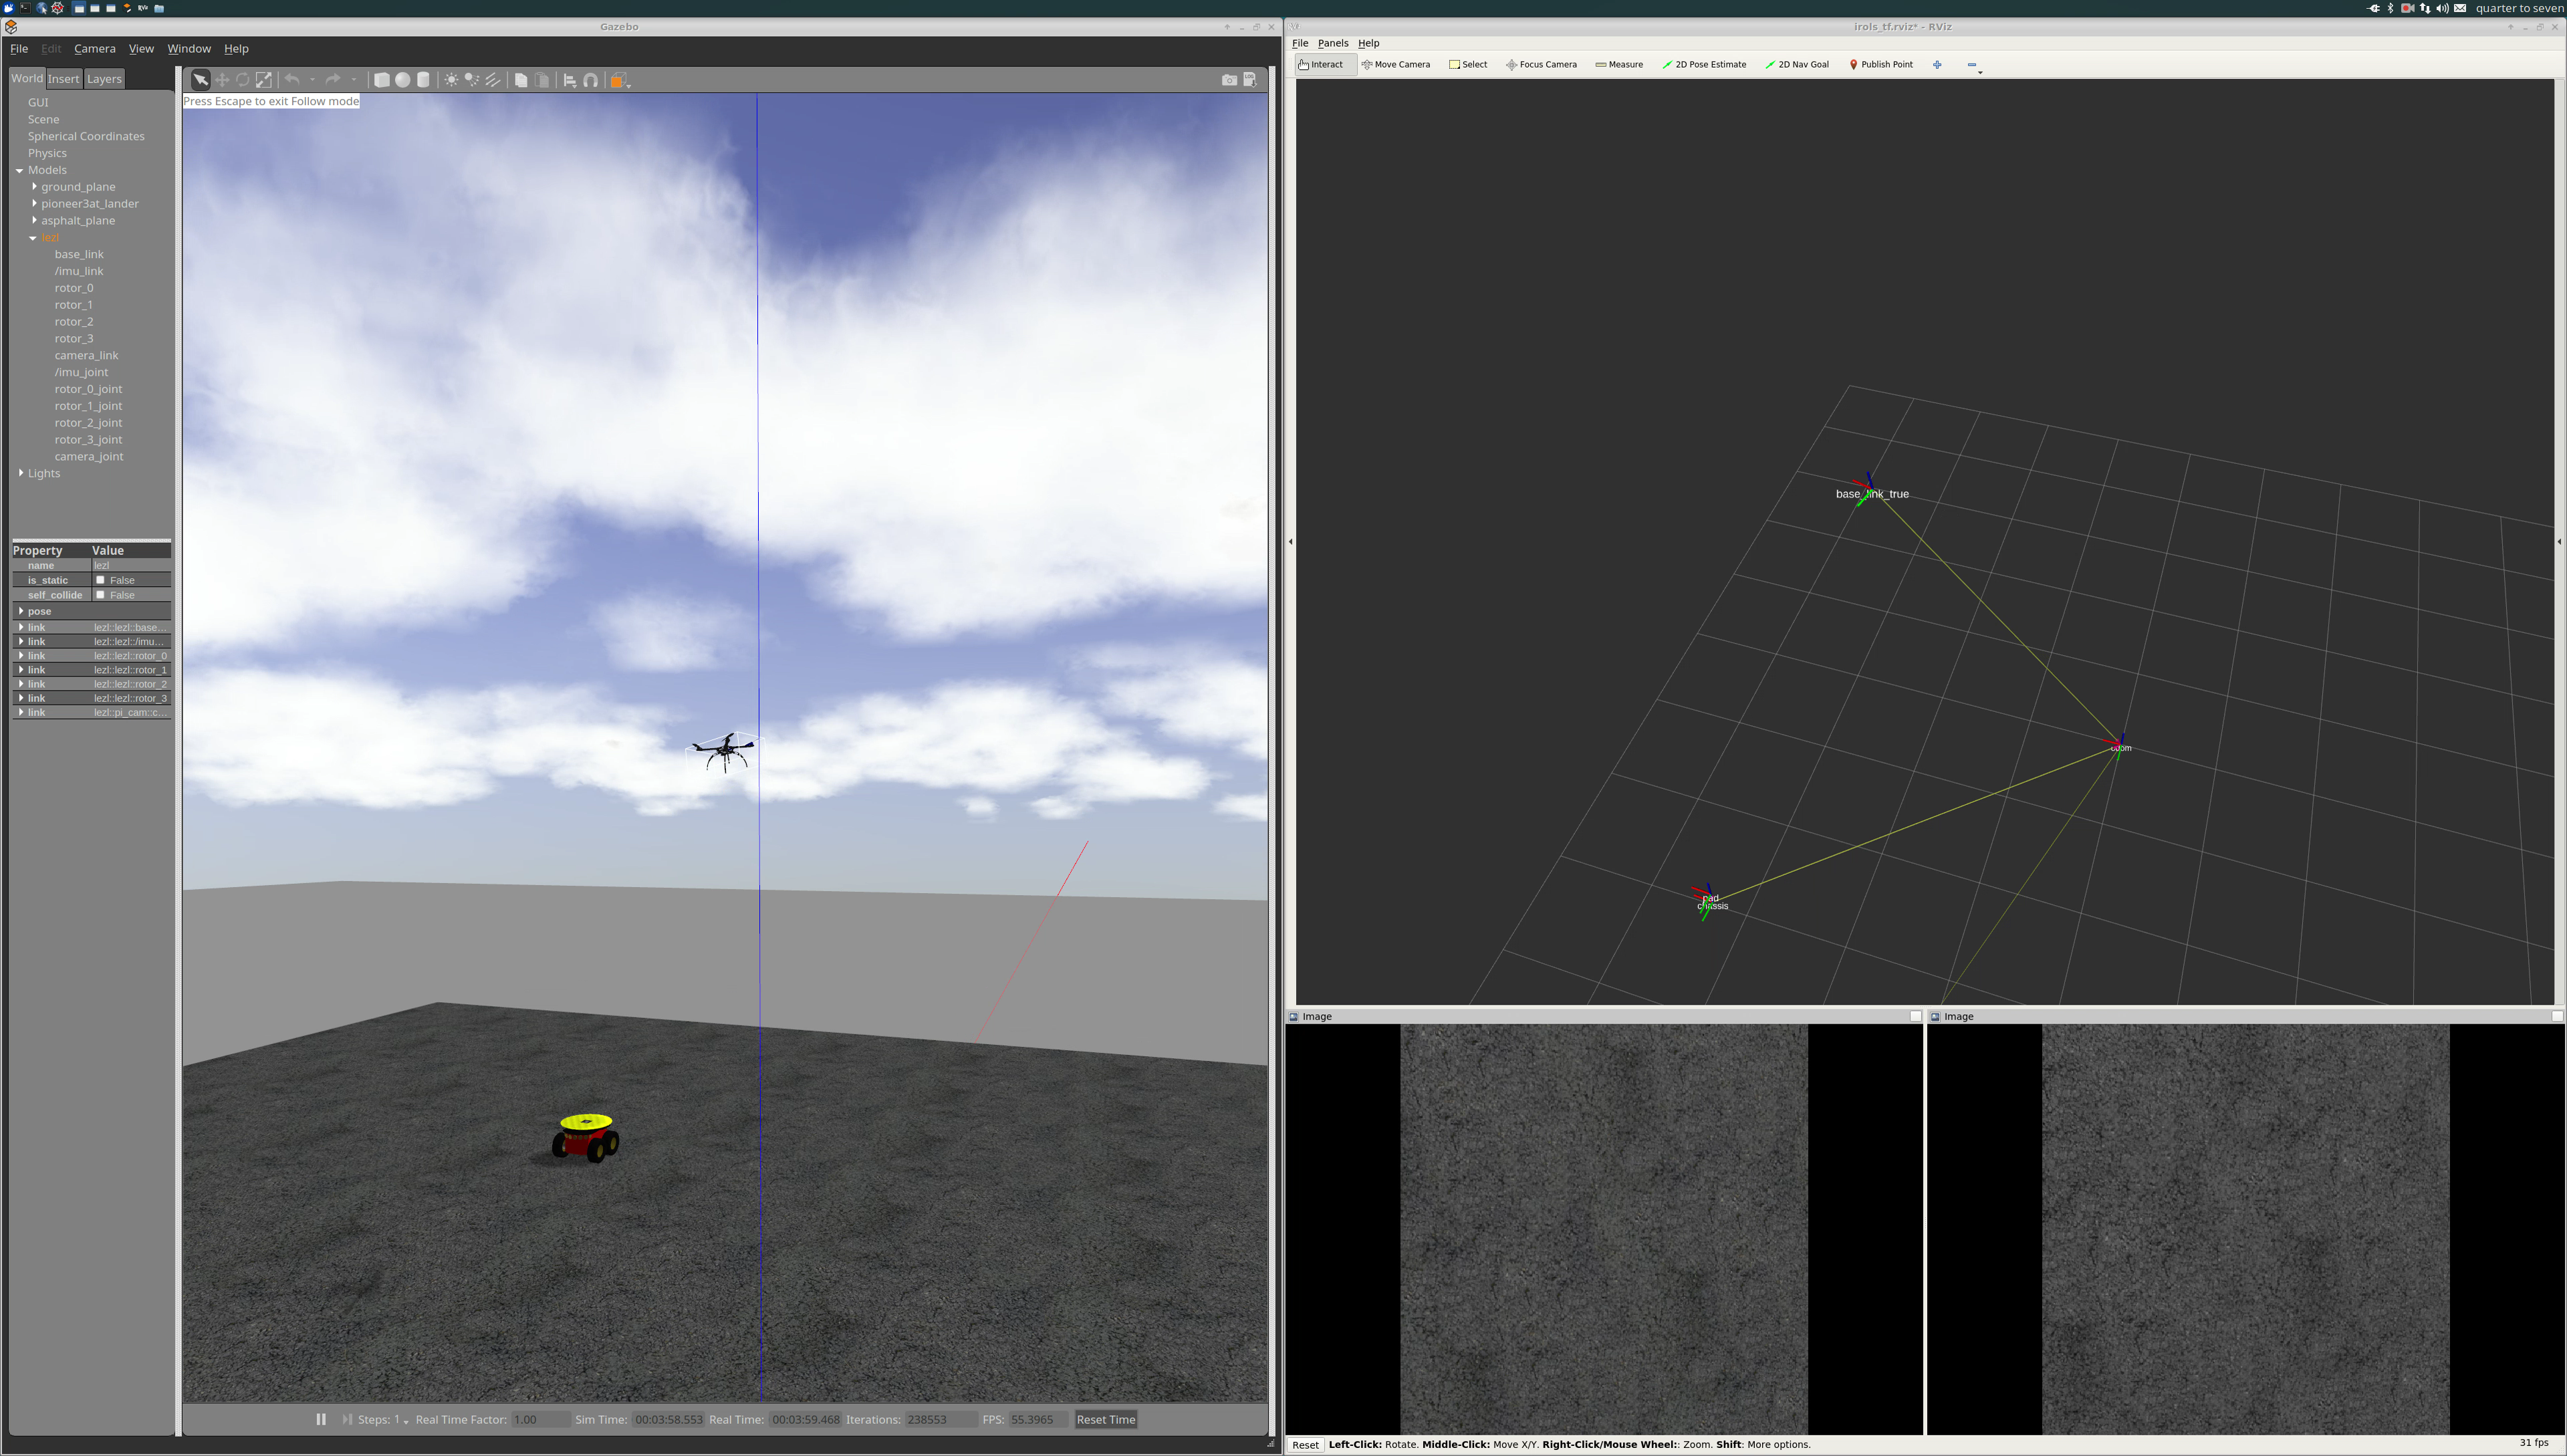
\includegraphics[width=0.90\textwidth]{images/moving_capture/moving-18h10m27s752}
    \caption{The vehicle before its camera has had an opportunity to image the target. Truth data is the only
    frame depicted in the coordinate transformation space.}\label{f:tf_truth}
\end{figure}

\begin{figure}
    \centering
    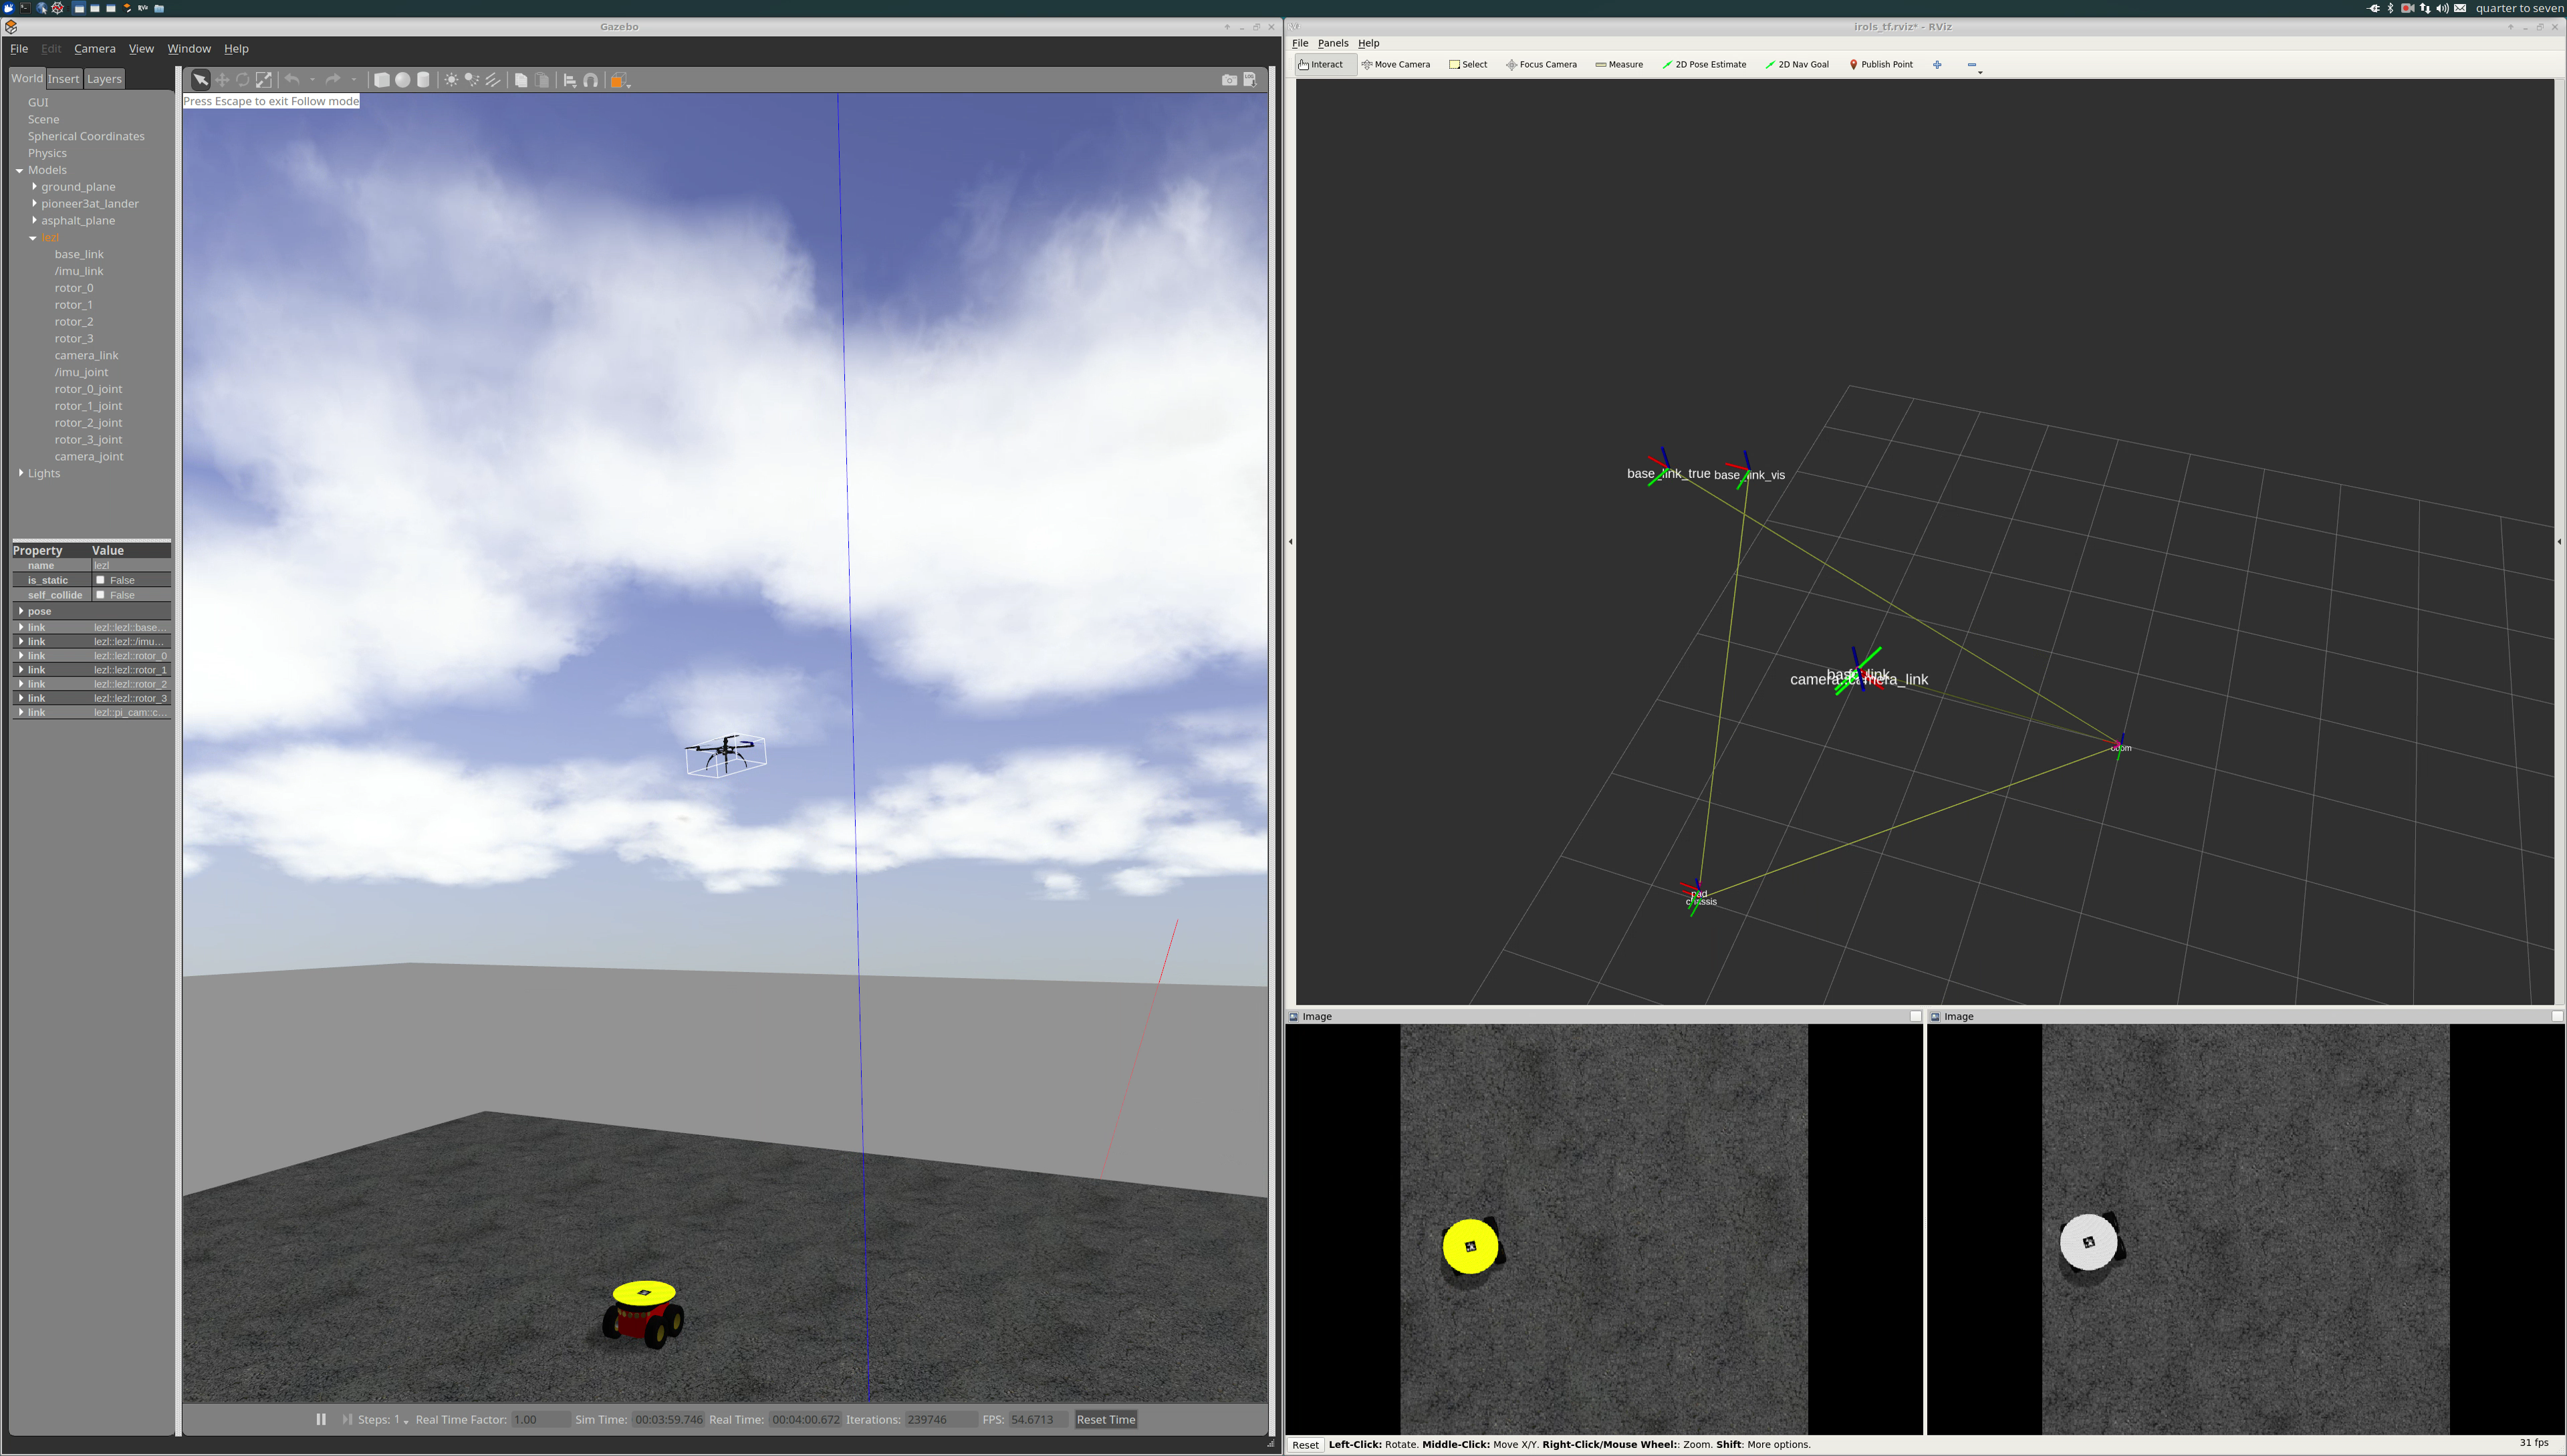
\includegraphics[width=0.90\textwidth]{images/moving_capture/moving-18h10m47s367}
    \caption{The state of the simulation shortly after the platform has come into view. Note that the platform
    is shown in the camera's image feed, but there is no AprilTag detection as the vehicle is too far away to
resolve the tag. The EKF coordinate frame is now visible, but not yet stable. Note that the visual estimate
frame is a child of the platform frame.}\label{f:tf_visual}
\end{figure}

\begin{figure}
    \centering
    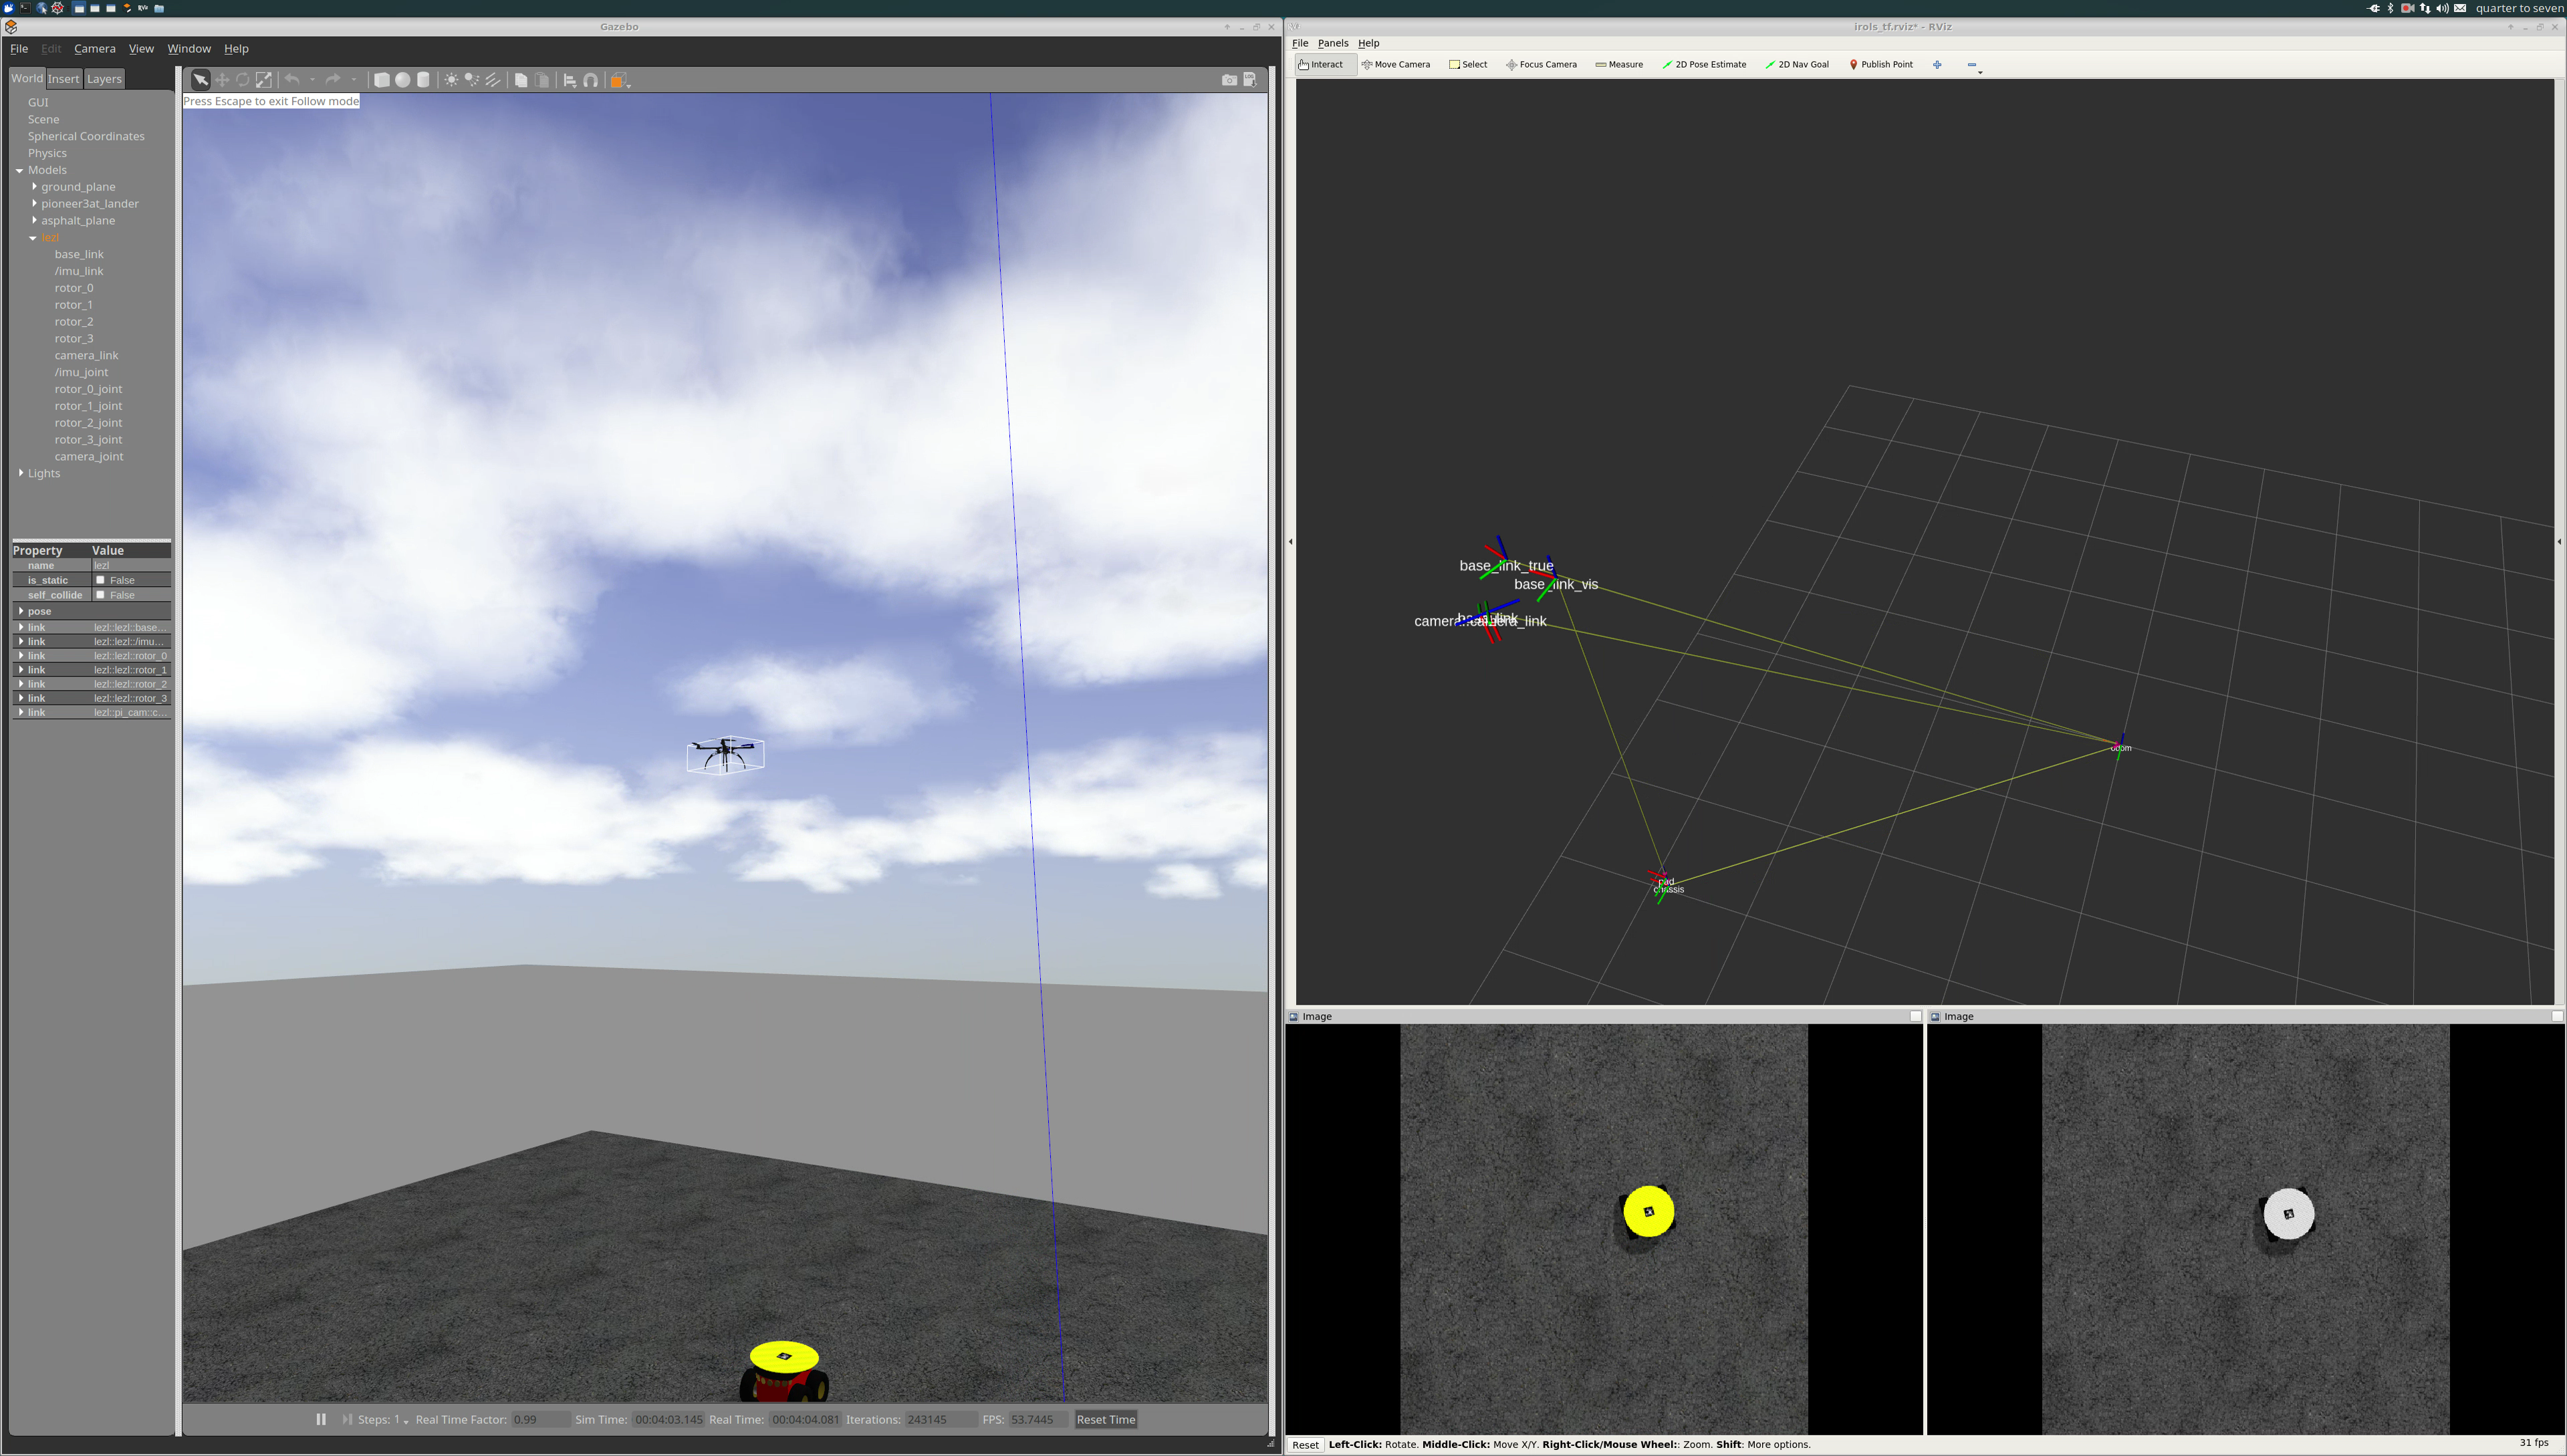
\includegraphics[width=0.90\textwidth]{images/moving_capture/moving-18h11m05s017}
    \caption{After some small amount of time, the EKF estimate has now started to converge onto truth data,
        but still shows large error as the visual estimate from the camera is the only input as of
    yet.}\label{f:tf_visual2}
\end{figure}

\begin{figure}
    \centering
    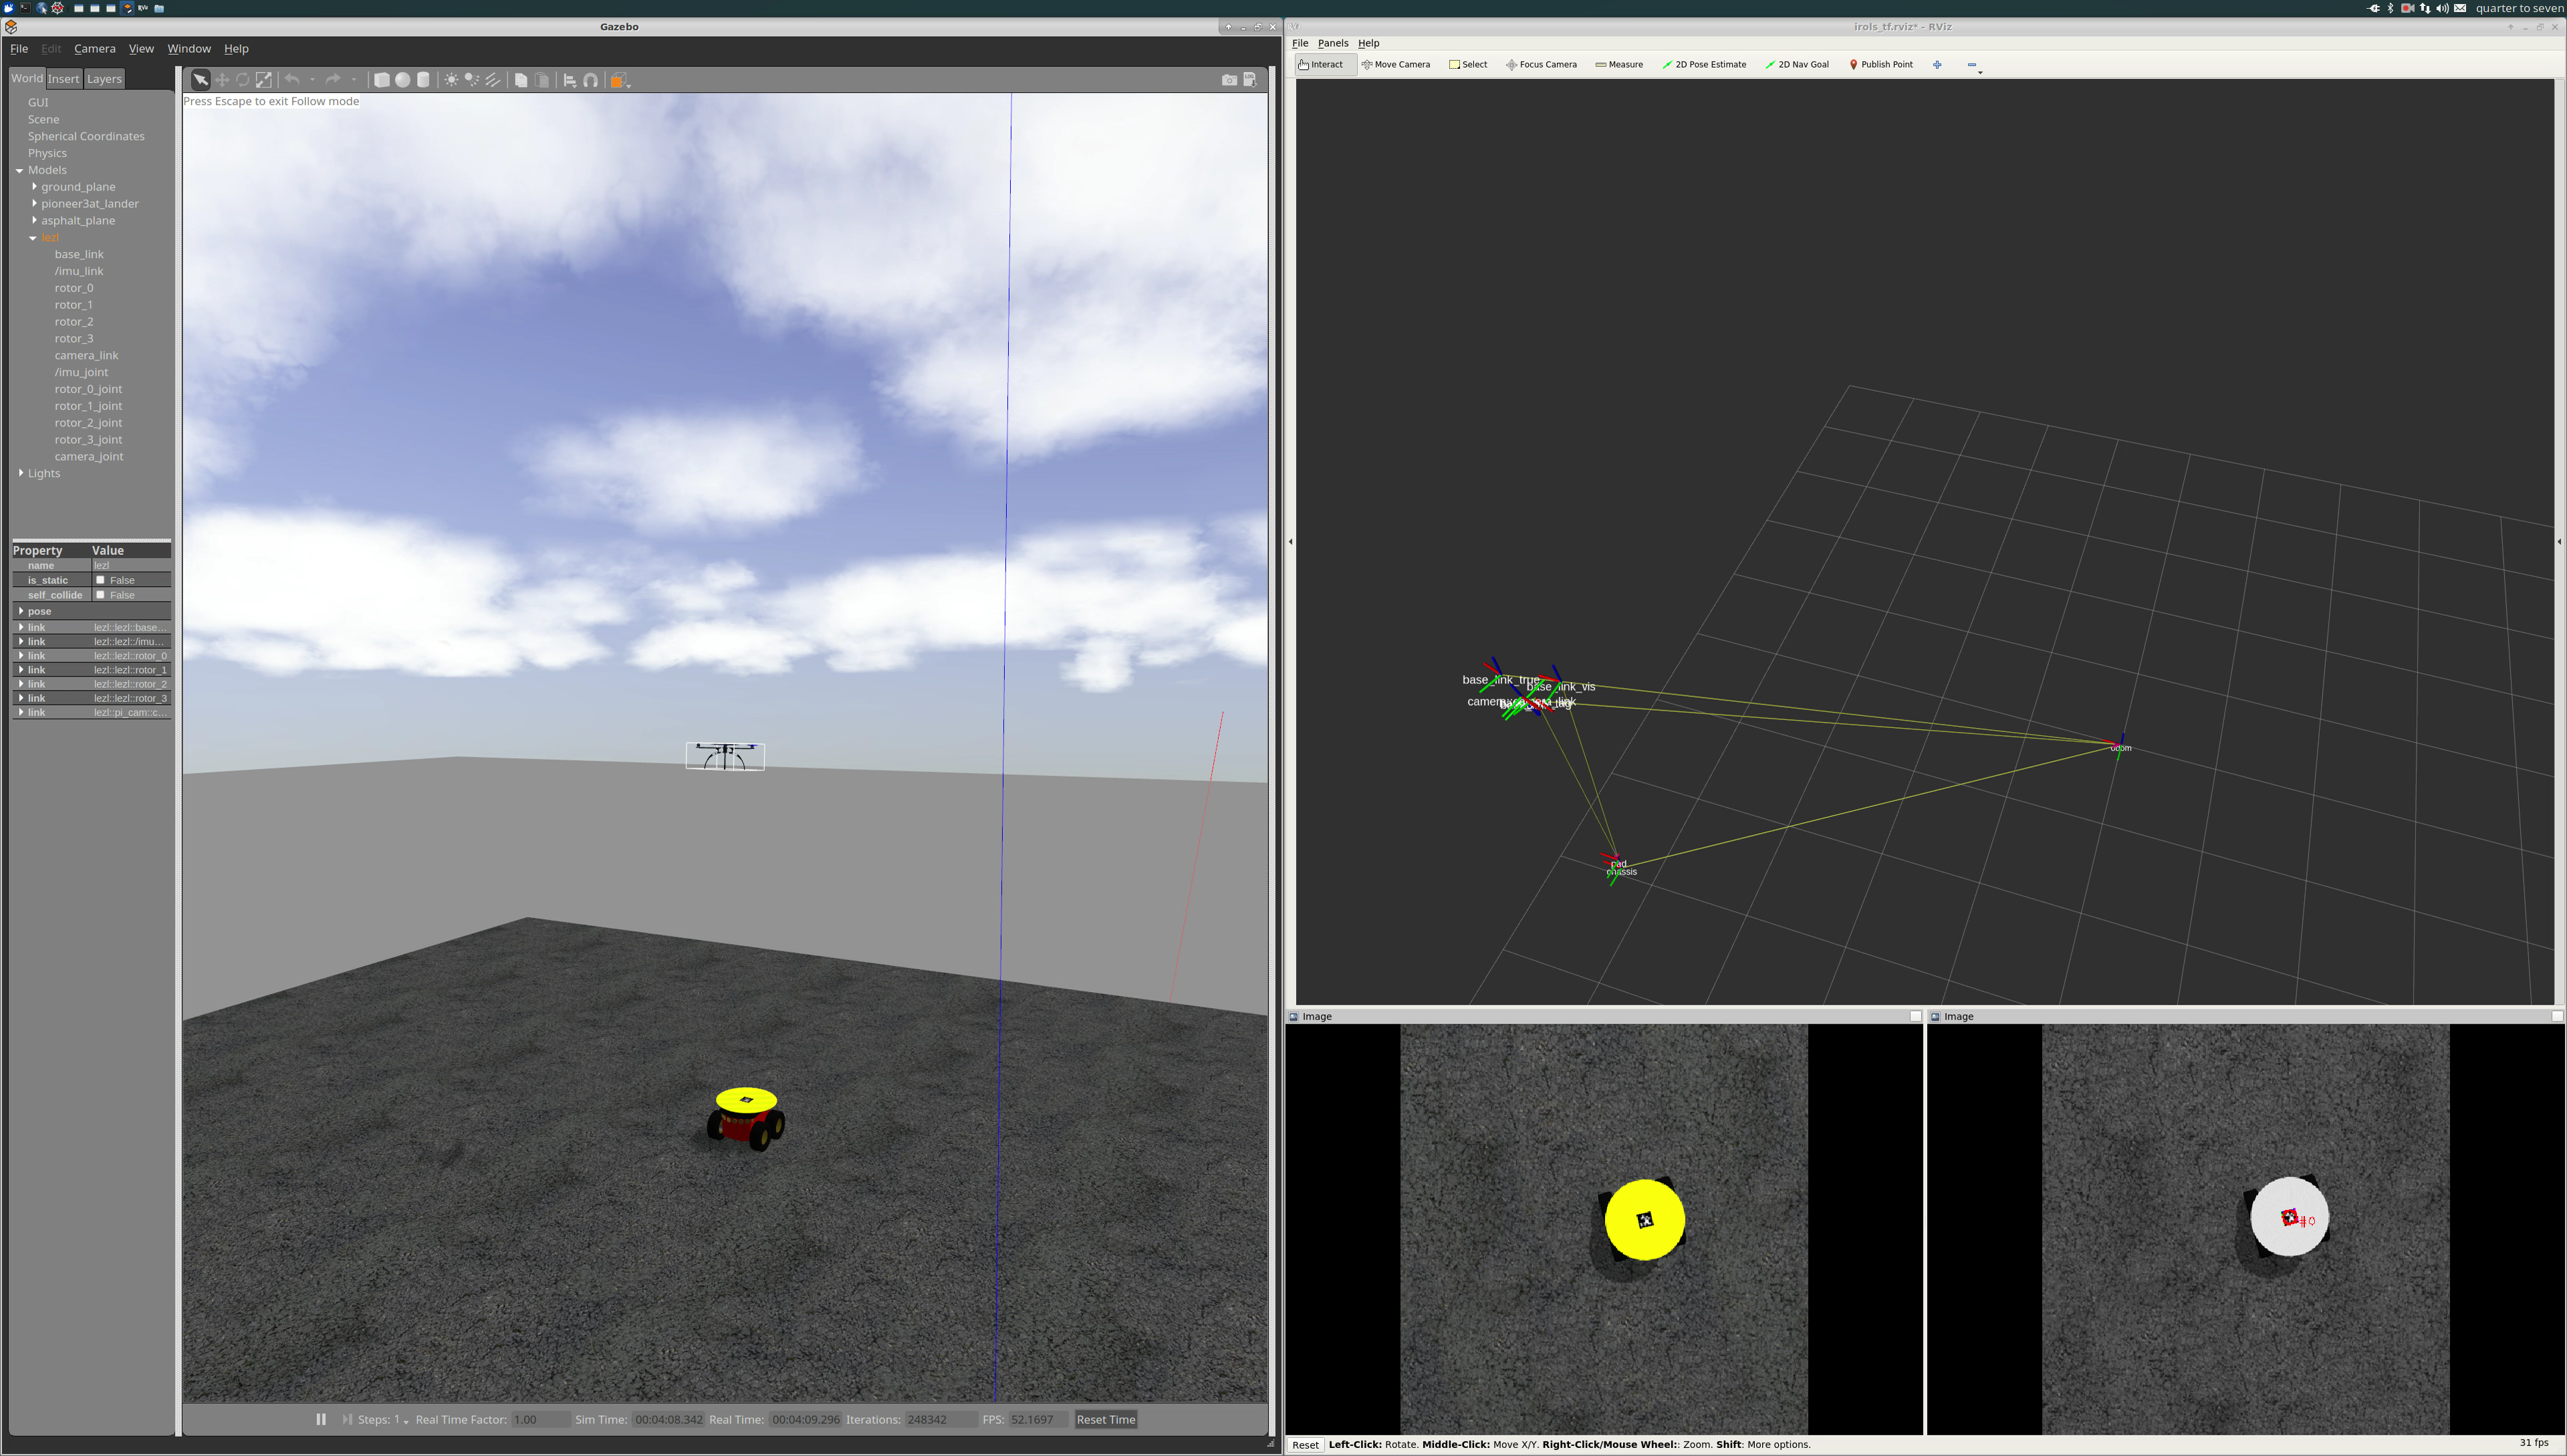
\includegraphics[width=0.90\textwidth]{images/moving_capture/moving-18h44m18s729}
    \caption{The AprilTag has now returned a detection and the EKF estimate is likewise converging towards
    truth with two estimate to fuse together.}\label{f:tf_april}
\end{figure}

\begin{figure}
    \centering
    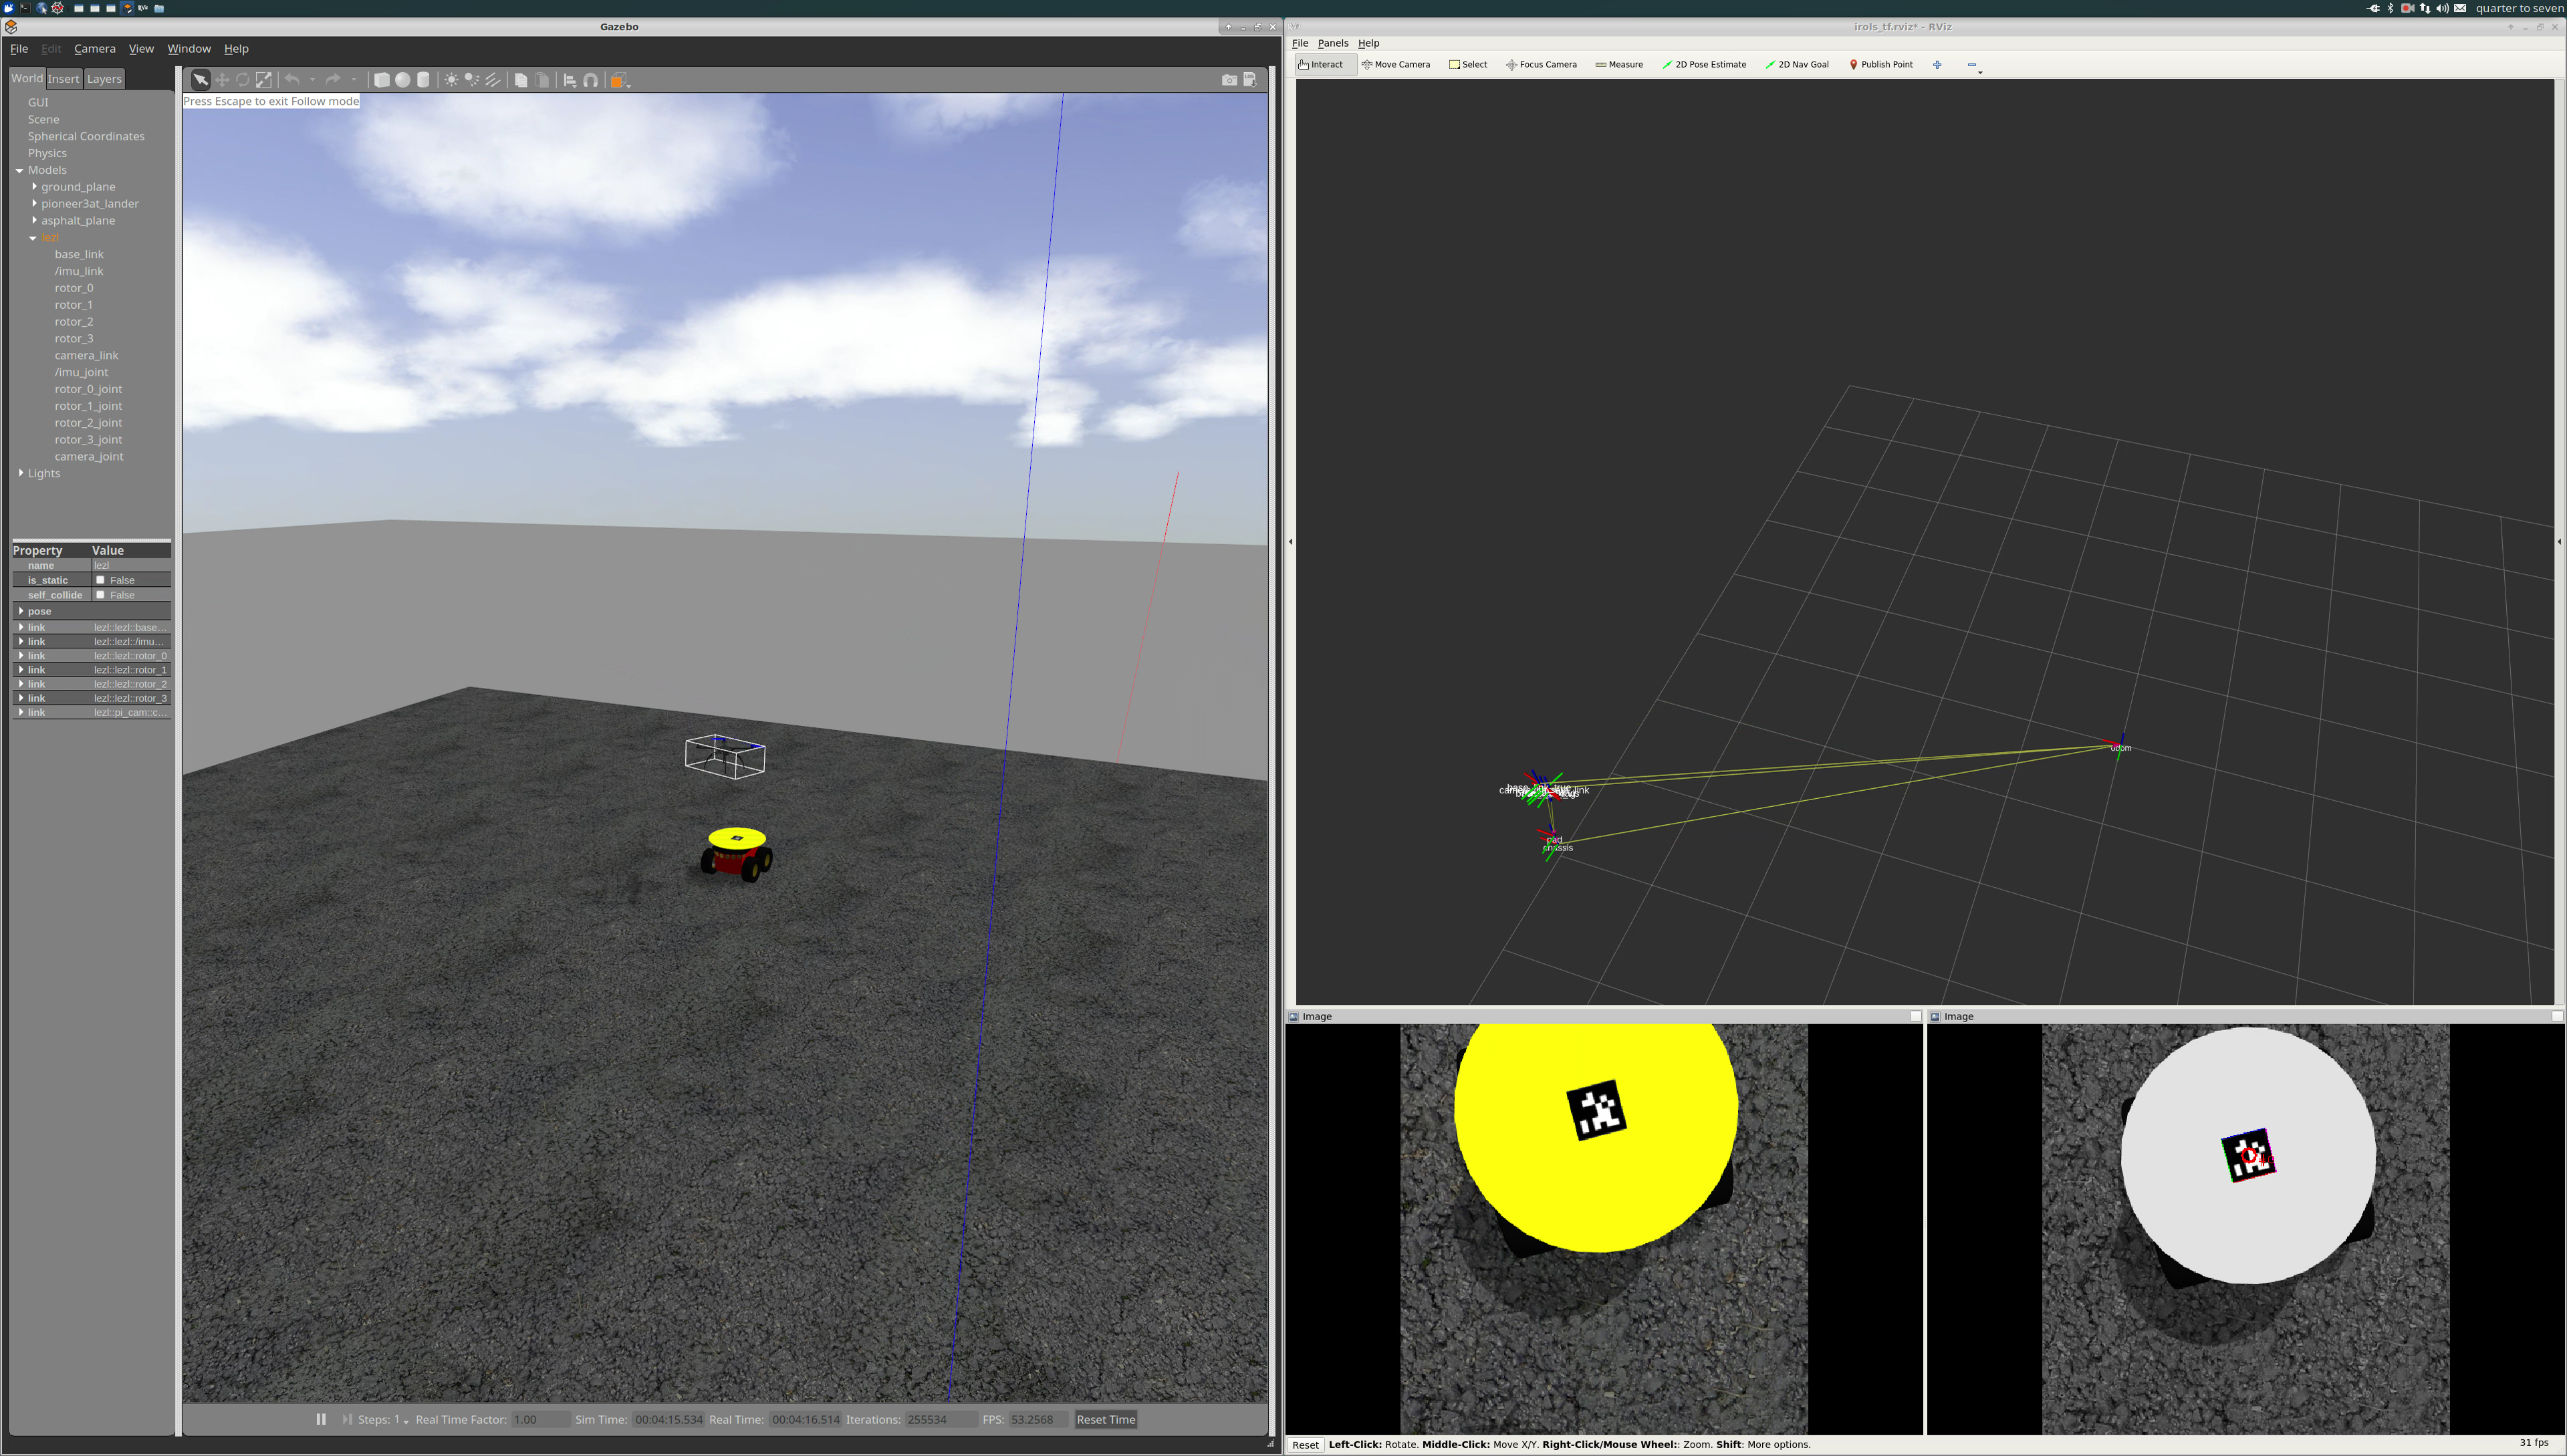
\includegraphics[width=0.90\textwidth]{images/moving_capture/moving-18h12m15s888}
    \caption{The simulation state just before the landing sequence has completed. The estimates at this range
    are very reliable.}\label{f:tf_final}
\end{figure}


